\documentclass[12pt,a4paper]{article}
\usepackage[utf8]{inputenc}
\usepackage[T1]{fontenc}
\usepackage{amsmath}
\usepackage{amsfonts}
\usepackage{amssymb}
\usepackage{multicol}
\usepackage{qrcode}
\usepackage{lmodern}
\usepackage{colortbl}%permet de griser les cases
\usepackage{tabularx, multirow}
%\usepackage{lscape}
\usepackage{xcolor}
%\usepackage{graphicx}
\usepackage{tikz,tkz-base}
\input{preambulemanu.sty}
\usepackage[left=2cm,right=2cm,top=2cm,bottom=2cm]{geometry}
\def\Oij{$\left(\text{O},~\vec{i},~\vec{j}\right)$}
\usepackage{fancyhdr}
\usepackage{MnSymbol,wasysym}

%Permet le code python sur lateX
\usepackage{minted}
\usemintedstyle{lovelace}



\begin{document}
\textbf{2nd} \hfill \textbf{Exercices vecteurs 2ème partie} \hfill Lycée Jean Rostand\\
\trait 

\subsection*{Exercice n°1}

Dans un repère, on donne les points:

$A(1;2)$\qquad $B(1;-4)$ \qquad $C(8;-6)$\\
Calculez les coordonnées des vecteurs $\vv{AB}$, $\vv{AC}$, $\vv{BC}$, $\vv{CA}$.

\subsection*{Exercice n°2}

Dans un repère, le point $A$ a pour coordonnées $(-1;3)$, le vecteur $\vv{u}$ a pour coordonnées $(3;-2)$.\\
$B$ est le point tel que $\vv{AB}=\vv{u}$.
Calculez les coordonnées de $B$.

\subsection*{Exercice n°3}

Dans un repère, on donne les points:

$A(-5;3)$\qquad $B(2;-2)$ \qquad $C(7;0)$\\

\begin{enumerate}
    \item 
    \begin{enumerate}
        \item Calculez les coordonnées des vecteurs $\vv{AB}$ et $\vv{AC}$
        
    \end{enumerate}
\end{enumerate}




\subsection*{Exercice n°1}

Dans le plan rapporté à un repère orthonormé \Oij{}, on considère les points $A$,$B$,$C$ et $D$.

\begin{center}
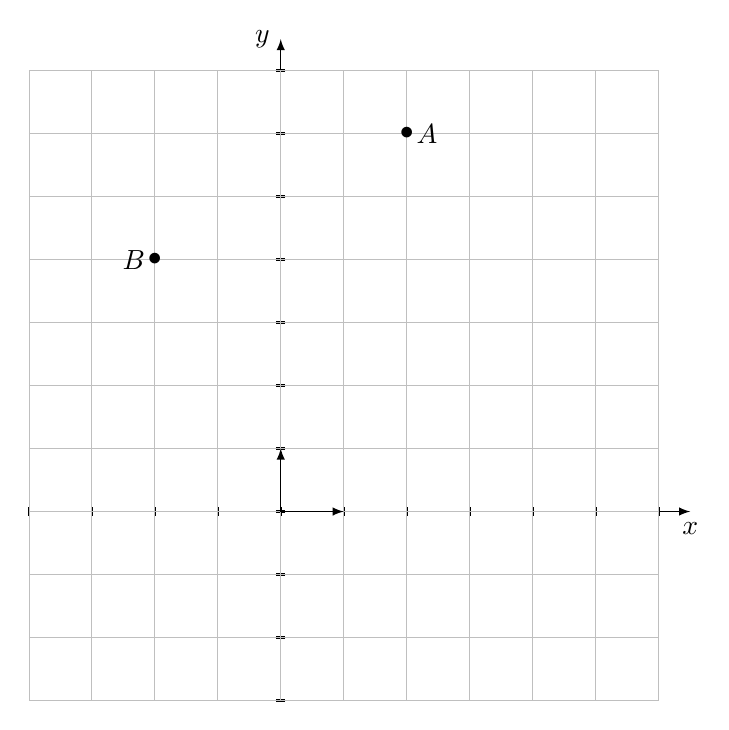
\begin{tikzpicture}[scale=0.8]
    \tkzInit[xmin=-4, xmax=6, ymin=-3,ymax=7]
    \tkzDrawXY
    \draw[lightgray,very thin] (-4,-3) grid (6,7);
    \draw [->,>=latex] (0,0) -- (1,0);
    \draw [->,>=latex] (0,0) -- (0,1) ;
    \draw (-2,4) node [left] {$B$};
    \draw (-2,4) node {$\bullet$};
    \draw (2,6) node [right] {$A$};
    \draw (2,6) node {$\bullet$};
\end{tikzpicture}
\end{center}

\begin{enumerate}
    \item Quelles sont les coordonnées de $A$ et $B$ ?
    \item Placer les points $C(1;-2)$ et $D(5;0)$
    \item 
    \begin{enumerate}
        \item Montrer que le vecteur $\vv{AD}$ a pour coordonnées $(3;-6)$
        \item Calculer les coordonnées du vecteur $\vv{BC}$
        \item Que peut-on en déduire quant à la nature du quadrilatère $ABCD$ ?
    \end{enumerate}
    \item Démontrer que $ABCD$ est un rectangle
    \item Déterminer les coordonnées du centre $M$ du rectangle $ABCD$
    \item On appelle \textbf{format} $r$ d'un rectangle le rapport: $r=\dfrac{longueur}{largeur}$. Déterminer le format du rectangle $ABCD$.
    \item 
    \begin{enumerate}
        \item Construire le point $E$ tel que $\vv{AE}=\dfrac{1}{r}\vv{AD}$
        \item Construire le point $F$ tel que $\vv{BF}=\dfrac{1}{r}\vv{BC}$
        \item Quelle conjecture peut-on émettre sur la nature que quadrilatère $ABFE$ ?
    \end{enumerate}
\end{enumerate}

\subsection*{Exercice n°2}


\end{document}
